\chapter{Task 3}
\begin{parlist}
	\item
	\renewcommand{\labelenumii}{\arabic{enumi}.\arabic{enumii}}
\renewcommand{\labelenumiii}{\arabic{enumi}.\arabic{enumii}.\arabic{enumiii}}
\renewcommand{\labelenumiv}{\arabic{enumi}.\arabic{enumii}.\arabic{enumiii}.\arabic{enumiv}}
\begin{center}
\begin{tabular}{ | m{8em} | m{32em} | } 
  \hline
  usecase & Webshop \\
  \hline
  Description & A company wants to use the Database in a webshop to check if they can sell a product to a customer\\
  \hline
  Actors & Customer company-employee/website  \\
  \hline
  Assumptions & the product data is stored in the database, the data in the database is accurate \\
  \hline
  Steps & \begin{enumerate}
        \item Webserver recieves purchase request
        \item Webserver sends query to database
        \item webserver recieves answer from database
        \item IF stock of the requested product is greater than 1
        \begin{tabular}{ c c }   
            THEN & 
            \item webserver continues purchasing process\\
            ELSE & webserver rejects request \\
        \end{tabular}
    \end{enumerate} \\
  \hline
  Variations & The webserver could check if the user has already bought x of the product and reject their offer according to a x per person policy \\
  \hline
  Non-Functional & The database must be able to handel multiple queries at once in order to process multiple orders at once \\
  \hline
  Issues &  \\
  \hline
\end{tabular}
\end{center}
	\item 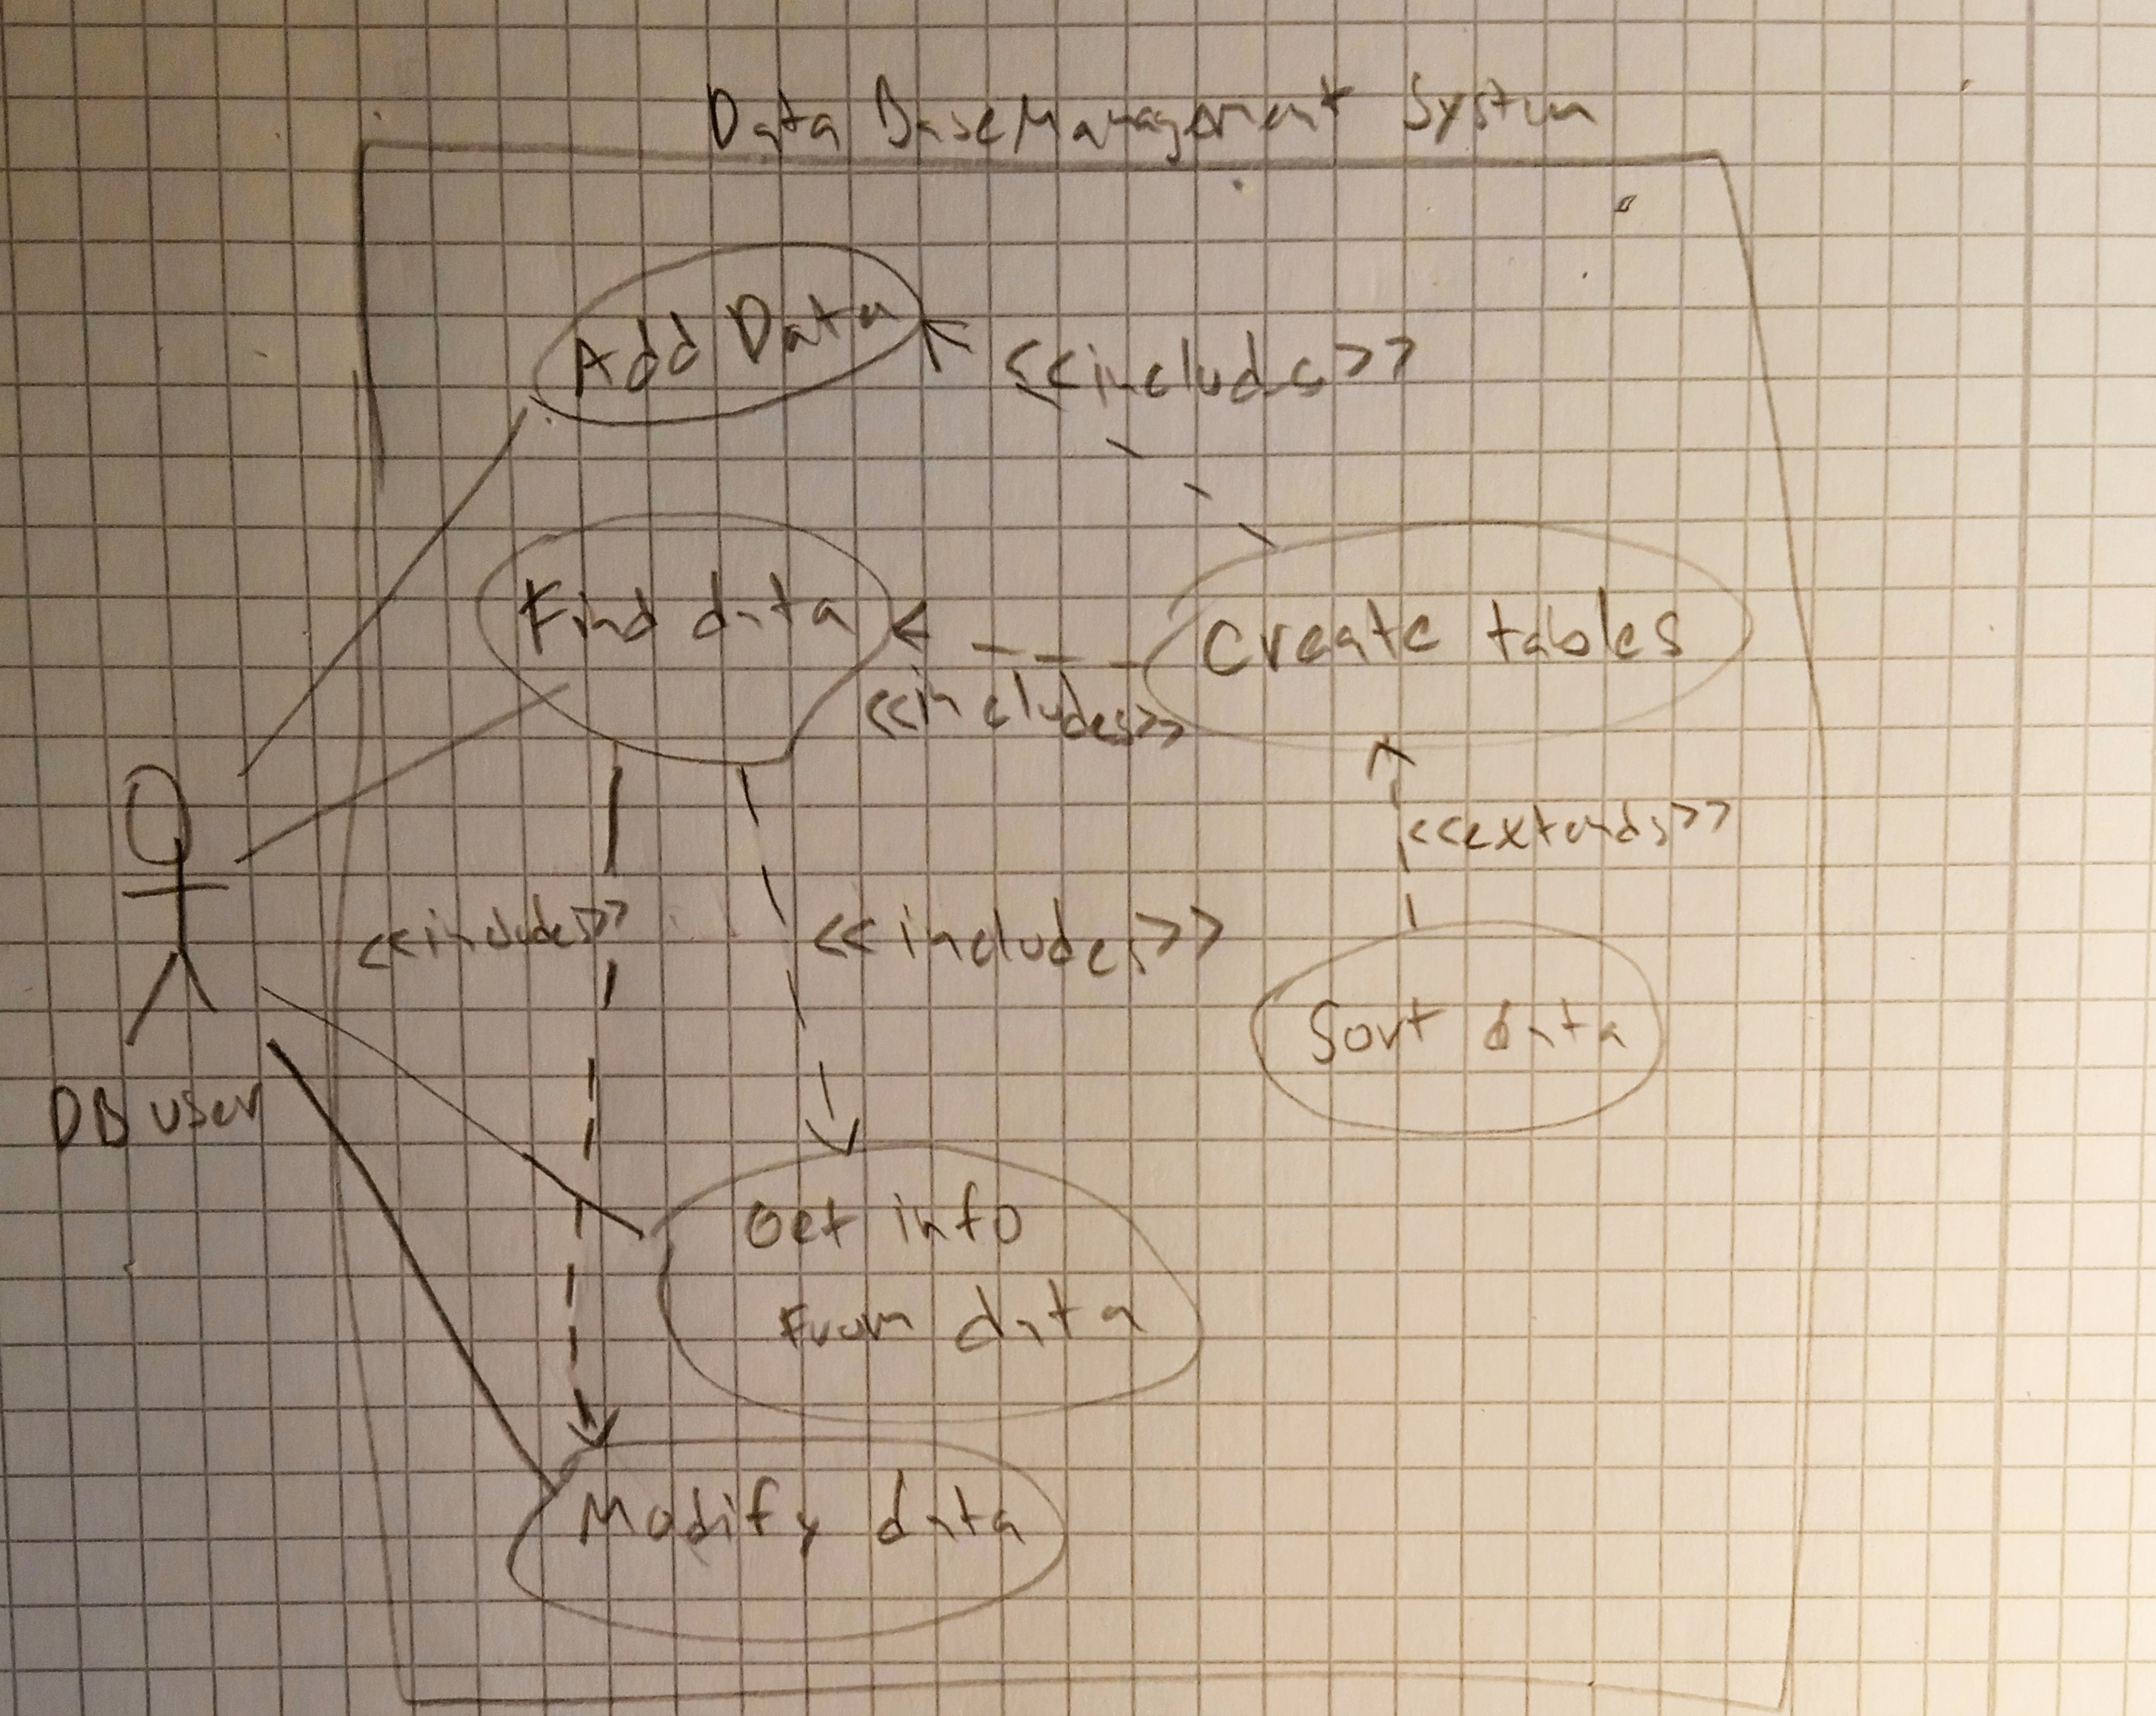
\includegraphics{IMG_20230520_192425}
\end{parlist}
